%%%%%%%%%%%%%%%%%%%%%%%%%%%%%%%%%%%%%%%%%%%%%%%%%
% Introduction AND Context
%%%%%%%%%%%%%%%%%%%%%%%%%%%%%%%%%%%%%%%%%%%%%%%%%

Irregularities in blood pressure are related to the exposure of some low-molecular biochemical elements ($<69$ kDa). For example, sodium, potassium, nitrates and some metal-mixtures are associated with high blood pressure in the general population \cite{yang_sodium_2011,mente_association_2014,elliott_intersalt_1996,smallwood_relationship_2017,siervo_inorganic_2013,
bondonno_absence_2015,carlstrom_dietary_2011,abhyankar_arsenic_2011}. Excretion of those elements in human urine is a reflection of their total exposure. Recently, a study reported that environmental agents, such as ambient air pollution and metal-mixtures, are underappreciated as risk factors for cadiovascular diseases such as hypertension that is an abnormally high blood pressure \cite{cosselman_environmental_2015}. Linear or logistic regressions are often used in order to determine the effect of biochemical elements on blood pressure \cite{yang_sodium_2011,mente_association_2014,elliott_intersalt_1996,smallwood_relationship_2017,jones_urine_2011}. However, multiple regression methods face three problems: 1) the tendency to make a true association statistically non-significant through multicollinearity; 2) the tendency to make a true association non-significant and smaller than it is through random measurement errors of covariates (regression dilution bias) as seen in the INTERSALT study where the effect of sodium on blood pressure was underestimated \cite{hutcheon_random_2010}; 3) difficulties in dissociating the effect of a predictor from that of a confounder. In order to account for this last point, supplementary variables and interactions are often added in the regression models, however the number of all possible interactions is often important and interpretation of interactions of the order of more than two is non-trivial. These three problems partially stem from the fact that the biochemical elements are intercorrelated. Firstly, correlations can be consequences of physiological processes. For example, potassium supplementation promotes sodium retention and potassium loss \cite{adrogue_sodium_2014}. Secondly, dietary patterns can induce correlations between molecules. For example, both nitrate and potassium are known to decrease blood pressure in the general population and both come from a diet rich in fruits and vegetables \cite{smallwood_relationship_2017}.

Since clustering puts in evidence patterns of biochemical elements rather than elements taken alone, we think that clustering methods can mitigate these problems. For example, clustering is applied to metabolomics to learn how biochemical patterns from urine or blood samples can be associated with dietary patterns \cite{osullivan_dietary_2011}. We think that clustering and dimentionality reduction have the potential to better predict hypertension in regression in addition to a better visual summary of the data.

To test these hypotheses, we will use the data from the Swiss Kidney Project on Genes in Hypertension (SKIPOGH) which is a Swiss study collecting medical data. Firstly, we will use principal component analysis (PCA) and cluster analysis to see if we can distinguish heterogenous groups of individuals in the data. The emerging principal components and biochemical clusters are expected to be meaningful in terms of physiological processes and dietary patterns. Then, we will see how these exploratory findings are associated (or not) with hypertension. We will perform regression both for hypertension status (binary variable) and blood pressure (continuous variable). 

We will also construct regression models with observed covariates and compare their results with the methods mentioned above.

Note that all the analysis was conducted in \texttt{R version 3.5.0} (2018-04-23) using the packages \texttt{``FactoMineR''} version 1.41 for PCA and \texttt{``cluster''} version 2.0.7-1 for PCA and cluster analysis, respectively.

In the following chapter called \emph{Context}, we present some biomedical notions that can be useful for the interpretation of the results. The subsequent chapters relate directly to the statistical analyses: \emph{Data description and preprocessing}, \emph{Methods} and \emph{Results}. R-code and abbreviations glossary are shown in the \emph{Appendix}.

%%%%%%%%%%%%%%%%%%%%%%%%%%%%%%%%%%%%%%%%%%%%%%%%%
% Context
%%%%%%%%%%%%%%%%%%%%%%%%%%%%%%%%%%%%%%%%%%%%%%%%%

\chapter{Context}
\label{ch:Context}

\section{An overview of hypertension}
In 2005, Kearney et al. estimated the worldwide prevalence of hypertension \cite{kearney_global_2005}. They combined reported prevalences of hypertension in 31 articles published from 1980 to 2002. Using demographic data as auxiliary variables, the worldwide prevalence in 2000 was estimated at $26.4\%$ (95\% Confidence Interval, abbrev. 95\% CI, was 26.0-26.8\%) by age and sex using post-stratification. Using extrapolation from Taylor series approximation methods, the projected prevalence for 2025 was $29.2\%$ ($95\% \text{ CI } 28.8-29.7\%$) \cite{kearney_global_2005}. An article published in the medical journal \emph{The Lancet} in 2002, concluded that hypertension is the leading risk factor for mortality and is ranked third as a cause of disability-adjusted life-years, which is a measure of morbidity \cite{ezzati_selected_2002}. Hypertension belongs to the Metabolic Syndrome which is defined by the authors of \emph{Harrisons Principles of Internal medicine} as ``a constellation of metabolic abnormalities that confer increased risk of cardiovascular disease and diabetes mellitus'' (Table \ref{table:metabolic}) \cite{kasper_harrisons_2015}. Consequently, the exploration of risk factors for hypertension is a critical step in the prevension of hypertension, and more generally a public health issue.

\section{Measuring and defining hypertension}
The \emph{sphygmomanometer} is an instrument which measures blood pressure expressed in \emph{mmHg} (see Figure \ref{fig:sphyngo}). The instrument gives two values: the \emph{systolic pressure} (SBP) and the \emph{diastolic pressure} (DBP) that are respectively the blood pressure during cardiac muscle contraction (systole) and the blood pressure during cardiac muscle relaxation (diastole). The SBP is always greater than the DBP. The bivariate result is conventionally presented under the form SBP/DBP. For example, an individual with SBP=130 and DBP=80 has a bivariate result of 130/80.

\begin{figure}
\centering
\centering
\captionsetup{singlelinecheck = false, format= hang, justification=raggedright, font=small, labelsep=space}
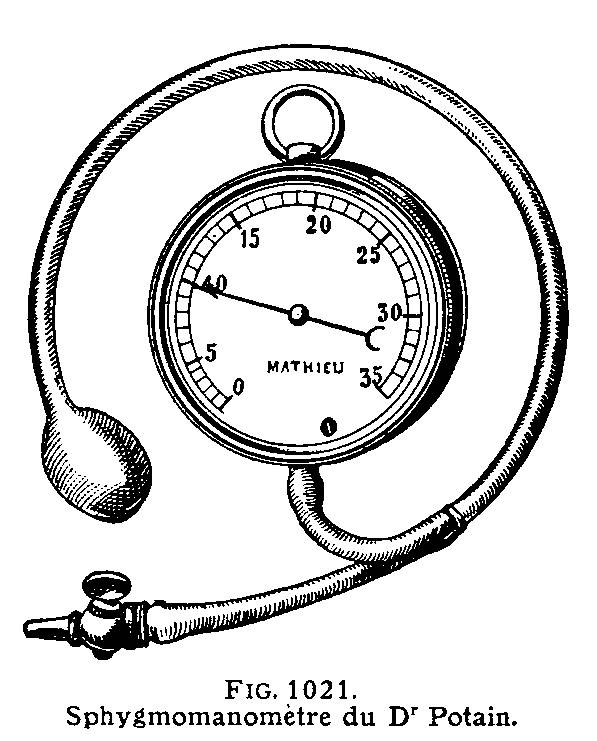
\includegraphics[width=0.45\linewidth]{sphyngo_01}
\captionof{figure}{Historical sphygmomanometer.}
  \label{fig:sphyngo}
\begin{flushleft}
{\footnotesize \emph{Larousse médical illustré}, 1912. Ed. Librairie Larousse, Paris \cite{galtier-boissiere_larousse_1912}.}
\end{flushleft}
\end{figure}

Hypertension is defined as a SBP greater than 140 mmHg, a DBP greater than 90 mmHg and/or use of antihypertensive medication \cite{kearney_global_2005,kearney_worldwide_2004}. This accepted definition allows for comparisons between different studies. 

So, hypertension can be expressed either as a binary variable using the definition above (presence of hypertension or absence of hypertension) or as a continuous variable (values of SBP/DBP). Thereby, a wide range of different statistical models can be used to model hypertension. The binary variable contains much less information than the continuous variable because of dichotomization. Consequently, the dichotomized variable can loose information useful in statistical analyses. On the other hand, the binary variable is often more meaningful from a clinical point of view (increased cardiovascular risk and decision boundary for treatment).

\begin{table}
\centering
\small
\captionof{table}{Definition Criteria for the Metabolic Syndrome \cite{kasper_harrisons_2015}.}
\begin{tabular}{ p{0.75\linewidth - 2\tabcolsep} }
\toprule
\bf{Three or more of the following:} \\
\begin{itemize}
\item Central obesity: waist circumference $>102$ cm (M), $>88$ cm (F) 
\item Hypertriglyceridemia: triglyceride level $\geq 150$ mg/dL or specific medication 
\item Low HDLc cholesterol: $<40$ mg/dL and $<50$ mg/dL for men and women, respectively, or specific medication 
\item Hypertension: blood pressure $\geq 130$ mmHg systolic or $\geq 85$ mmHg diastolic or specific medication 
\item Fasting plasma glucose level $\geq 100$ mg/dL or specific medication or previously diagnosed type 2 diabetes 
\end{itemize} \\
\bottomrule
\end{tabular}
\label{table:metabolic}
\end{table}

\section{Biochemical elements}
For the purpose of this study, we are interested in two families of potential risk factors for hypertension: the metal-mixtures and the non-metals. Both families are elements coming from alimentation and/or environmental exposure, and are described in detailed in this section.

\subsection{Metallome}
According to the definition by Joanna Szpunar, the \emph{metallome} is ``\emph{the entirety of metal and metalloid species \footnote{metal-mixtures: metals and metalloids} within a cell or tissue type}'' \cite{szpunar_advances_2005}. Although metals and metalloids are toxic for the human body in many cases, they are necessary for physiological processes in some cases. A classical exemple of an essential metal is iron whose deficiency leads to anemia in 2\% of the adult population \cite{iron_anemia}. Exposure can come from water, food, air, medications and even dietary supplements.

Metals are present in the left part of the \emph{periodic table of elements} (see Figure \ref{fig:periodic_table}). They share sharing some characteristics that distinguish them from other elements, such as the as ability to conduct electricity, a metallic shine, malleability and ductility. These four characteristics result from the high mobility of electrons in metals \cite{atkins_chimie:_2007}.

Some chemical elements between the metals and the nonmetals in the periodic table are classed as metalloids. They have some --- but not all --- metallic characteristics.

Table \ref{table:des_metallome} presents some of the metals and metalloids most relevant to public health.

\begin{figure}
\centering
\captionsetup{singlelinecheck = false, format= hang, justification=raggedright, font=small, labelsep=space}
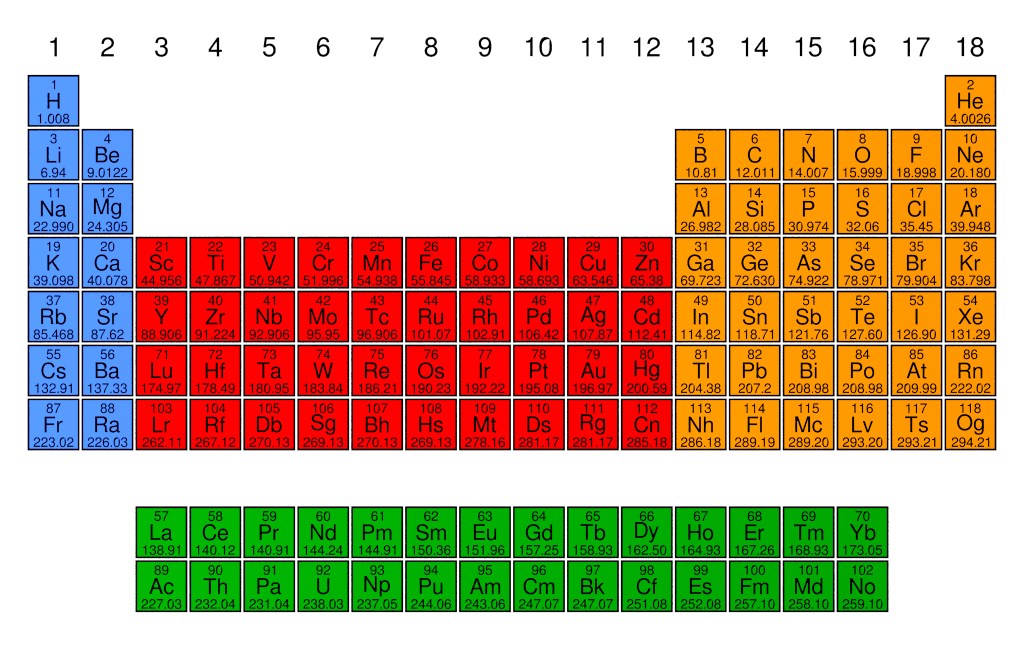
\includegraphics[width=0.75\linewidth]{periodic_table_standard}
\captionof{figure}{Periodic table of elements.}
  \label{fig:periodic_table}
\begin{flushleft}
{\footnotesize \textbf{Metals} are in the blue, red, green and in the lower left orange groups. \textbf{Metalloids} are the elements in the diagonal of the orange square, i.e. Boron, Silicon, Germanium, Arsenic, Antimony, Tellurium. \\
\emph{Source: www.webelements.com}}
\end{flushleft}
\end{figure}

\begin{center}
\small
\captionof{table}{Description of metal-mixtures of medical interest.}
\begin{longtable}{p{0.16\linewidth - 2\tabcolsep} p{0.16\linewidth- 2\tabcolsep} p{0.16\linewidth- 2\tabcolsep} p{0.51\linewidth - 2\tabcolsep}}
\hline
Element, \par \emph{chemical group}& Chemical \par symbol & Essential \par versus \par toxic & Medical interest \\
\hline
\endfirsthead
\multicolumn{4}{c}%
{\tablename\ \thetable\ -- \textit{Continued from previous page}} \\
\hline
Element, \par \emph{chemical group}& Chemical \par symbol & Essential \par versus \par toxic & Medical interest \\
\hline
\endhead
\hline \multicolumn{4}{r}{\textit{Continued on next page}} \\
\endfoot
\hline
\endlastfoot
Lithium, \par \emph{metal} & Li & Toxic & - Common drug for bipolar disorder \par - Renal toxicity and cardiac conduction disorders in high doses \\
Beryllium, \par \emph{metal} & Be & Toxic & - Professional exposure: processing alloys for high-tech industries \par - Lung diseases such as chronic granulomatous disease \\
Aluminum, \par \emph{metal} & Al & Toxic & - Aluminum oxyde hydrate as treatment for dyspepsia (historically) \par - Nowadays avoided because of the risk of acute dementia and bone fractures \par - Other sources are food (as preservative and coloring agent) and professional exposure but their contribution in total aluminum exposure is minor \cite{soni_safety_2001} \\
Vanadium, \par \emph{metal} & V & Toxic & - Deficiency could cause metabolic disorders \cite{panchal_selenium_2017} \par - New candidate drug for diabetes (animal models) \cite{tahrani_management_2011} \par - Could be considered as an essential metal-mixture \cite{wu_environmental_2018} \\
Chromium, \par \emph{metal} & Cr & Toxic & - Presence in food: yeast, meat, and grain products \par - Causing lung cancer \par - Professional exposure (bricklayers): presence in cement causing skin allergy \\
Manganese \par \emph{metal} & Mn & Essential & - Involved in human enzymes (like manganese superoxide dismutase) \par - Deficiency causing bone metabolism perturbations \\
Cobalt, \par \emph{metal} & Co & Essential & - Component of the cobalamine \par (Vitamin B12) \par - Vitamin B12 involved in DNA synthesis \\
Nickel, \par \emph{metal} & Ni & Toxic & - Professional exposure \par - Skin allergy \par - Potential carcinogen \cite{kasper_harrisons_2015} \\
Copper, \par \emph{metal} & Cu & Essential & - Presence in many human enzymes \par - Involved in iron metabolism, energy production and neurotransmitter \par synthesis \cite{kasper_harrisons_2015} \par - Kidney and liver failure in case of intoxication \\
Zinc, \par \emph{metal} & Zn & Essential & - Present in many human enzymes \par - Necessary for fetal growth and embryonic development \\
Arsenic, \par \emph{metalloid} & As & Toxic & - Historical poison \par - Professional exposure \par - Water contamination \par - Interferes with energy production \par - Presence in some drugs against leukemia \par - Can lead to death by organ toxicity and fluid loss \cite{kasper_harrisons_2015} \\
Molybdenum, \par \emph{metal} & Mo & Essential & - Present in human enzymes (sulfite and
xanthine oxidase) \par - Sometimes found in multimineral tablets \\
Palladium, \par \emph{metal} & Pd & Toxic & - Sources: jewellery and dental restorations \par - Contact allergy at sites of piercing or oral symptoms if dental restorations \cite{faurschou_metal_2011} \\
Silver, \par \emph{metal} & Ag & Toxic & \\
Cadmium, \par \emph{metal} & Cd & Toxic & - Professional exposure (smelting, battery and plastics industries) \par - Batteries and tobacco \\
Tin, \par \emph{metal} & Sn & Toxic & \\
Antimony, \par \emph{metalloid} & Sb & Toxic & \\
Platinum, \par \emph{metal} & Pt & Toxic & - Genotoxic (study on cells) \par - Augmentation of platinum group elements (PGE) during the last decades (combustion catalyst for cars) \par - Other sources: industries using PGE, hospitals and dental laboratories \cite{wiseman_airborne_2009} \\
Mercury, \par \emph{metal} & Hg & Toxic & - Professional exposure (ex. automobile and construction) \\
Thallium, \par \emph{metal} & Tl & Toxic & - Insecticides, metal alloys and fireworks \par - Severe poisoning can follow a single dose $>1$ g\\
Lead, \par \emph{metal} & Pb & Toxic & - Professional and domestic exposure \par - Food or water from improperly glazed ceramics \\
Bismuth, \par \emph{metal} & Bi & Toxic & - Prophylaxis of travelers’ diarrhea (approx. 60\% effective) \par - Effective drug for helicobacter pylori infection \\
\end{longtable}
\label{table:des_metallome}
\begin{flushleft}
{\footnotesize \textbf{Remark}: Of the 22 metal-mixtures, 5 can be considered essential metal-mixtures: manganese, cobalt, copper, zinc and molybdenum. \\ The main reference for this table is Kasper et al. 2015 \cite{kasper_harrisons_2015}.}
\end{flushleft}
\end{center}

\subsection{Non-metals}
In this work, \emph{non-metals} refers simply to biochemical elements that are not metal-mixtures. They include:
\begin{itemize}
\item Electrolytes: as defined by the second edition of \emph{Oxford Dictionary of Public Health}, an electrolyte is \emph{``an ion or compound derived from an element, such as sodium, potassium, or carbon, that when dissolved or suspended in a liquid medium transmits an electric current and is deposited on the positive or negative electrode, depending on whether the electrolyte is negatively or positively charged''}\cite{last_dictionary_2018}. 
\item Metabolites: products of metabolism (energy production).
\end{itemize}



